\documentclass{llncs} % ← 关键：使用 llncs 而不是 article

\usepackage{graphicx}
\usepackage{cite}
\bibliographystyle{splncs04}
 \usepackage{amsmath} 
% 必须加载 tikz 宏包
\usepackage{tikz}
% 加载 positioning 库以支持 right=of 等语法
\usetikzlibrary{positioning}
\usepackage{listings}
\usepackage{xcolor} % 可选，用于语法高亮配色
\usepackage{etoolbox} % 可选，用于修复某些兼容性问题
\usepackage{caption}

\usepackage{algorithm}
\usepackage{algpseudocode}

% 支持中文注释或 UTF-8（可选）
\usepackage[utf8]{inputenc}
\usepackage[T1]{fontenc}
\usepackage{lmodern}
\usepackage{amssymb}

\usepackage{xcolor}
\definecolor{codeblue}{rgb}{0,0,0.6}
\definecolor{codegreen}{rgb}{0,0.5,0}
\definecolor{codegray}{rgb}{0.5,0.5,0.5}
\definecolor{codepurple}{rgb}{0.58,0,0.82}
\definecolor{backcolour}{rgb}{0.98,0.98,0.98}

% 定义统一的代码样式
\lstdefinestyle{mystyle}{
    backgroundcolor=\color{backcolour},   
    commentstyle=\color{codegreen},
    keywordstyle=\color{codeblue}\bfseries,
    numberstyle=\tiny\color{codegray},
    stringstyle=\color{codepurple},
    basicstyle=\ttfamily\scriptsize, % 使用 scriptsize 稍微大一点点，也更清晰
    breakatwhitespace=false,         
    breaklines=true,                 
    captionpos=b,                    
    keepspaces=true,                 
    numbers=none,                    % 移除行号，让对比更清爽
    numbersep=5pt,                  
    showspaces=false,                
    showstringspaces=false,
    showtabs=false,                  
    tabsize=2,
    frame=single,                    % 统一加框
    framesep=3pt,                    % 框和代码的间距
    rulecolor=\color{black!30},      % 框的颜色稍微淡一点，不喧宾夺主
}

\lstset{style=mystyle}

\lstdefinelanguage{Rust}{
  keywords={%
    fn, let, mut, match, if, else, return, pub, struct, impl, trait, enum,
    use, mod, crate, self, super, as, dyn, static, const, unsafe, extern,
    type, where, async, await, move, ref, box, continue, break, loop, for,
    while, in, true, false
  },
  keywordstyle=\color{blue}\bfseries,
  ndkeywordstyle=\color{purple}\bfseries,
  identifierstyle=\color{black},
  sensitive=true,
  comment=[l]{//},
  morecomment=[s]{/*}{*/},
  commentstyle=\color{green!50!black}\ttfamily,
  stringstyle=\color{red}\ttfamily,
  morestring=[b]",
  morestring=[b]',
  basicstyle=\ttfamily\scriptsize,
  numbers=left,
  numberstyle=\tiny,
  frame=single,
  tabsize=4,
  showspaces=false,
  showstringspaces=false,
  escapeinside={(*@}{@*)}, % 可选：用于在代码中插入 LaTeX
}

% 定义 Coq 语言样式
\lstdefinelanguage{Coq}{
  % 第一组关键字：语言原语
  morekeywords={Inductive, Type, Definition, Fixpoint, match, with, end, forall, exists, Prop, Set, return, let, in},
  % 第二组关键字：自定义类型，用于加粗区分
  morekeywords=[2]{expr, pexpr, place, type, int, float, float32, int64, ident, unary_operation, binary_operation},
  sensitive=true,
  comment=[s]{(*}{*)},
  morecomment=[s]{(**}{*)},
  string=[b]",
  basicstyle=\ttfamily\tiny, 
  keywordstyle=\color{codeblue}\bfseries,
  keywordstyle=[2]\color{codeblue}, % 第二组关键字不加粗，仅上色
  commentstyle=\color{codegreen},
  stringstyle=\color{codepurple},
  breaklines=true,
  tabsize=2,
  showstringspaces=false,
  columns=flexible,
}

% LNCS 已内置双栏，无需额外设置

\begin{document}

\title{Clight2Rust: A Lightweight Framework for Translating a Subset of C to Safe Rust}

% 1. 作者列表
% 使用 \and 分隔
\author{Dongwen Yao \and Jinhua Wu \and Yuting Wang%% \thanks{Corresponding author.}
}

% 2. 页眉缩略名
\authorrunning{D. Yao et al.}

% 3. 机构信息
% 这里 \email 只填通讯作者的邮箱
\institute{Shanghai Jiao Tong University, Shanghai, China\\
\email{yuting.wang@sjtu.edu.cn}} % 

\maketitle


\begin{abstract}
Memory safety vulnerabilities in C programs remain a critical challenge in systems software. While rewriting legacy code in Rust offers a promising solution, manual migration is error-prone and labor-intensive. Existing automated translation tools either generate \texttt{unsafe} Rust or rely on heavy-weight static analysis that struggles with C's flexible pointer arithmetic.
%
We present a lightweight and automated approach to translating C to \emph{safe Rust} by exploiting dynamic lifetime and ownership checking provided by Rust's smart pointers.
%
Our method dynamically tracks ownership and borrow boundaries by using a novel pointer structure \texttt{Ptr<T>}, enabling the translation of complex C pointer operations---including aliasing and pointer arithmetic---into safe Rust code without relying on unsafe blocks in the generated user code, by combining a lightweight static analysis with dynamic checks. We implement our approach for the Clight subset of C, as defined in the CompCert verified compiler.
%
We implement our approach on top of intermediate languages designed for CompCert. Evaluation on a suite of benchmarks demonstrates that we translated all applicable test cases in CompCert's test suite, maintaining functional correctness (by comparing with GCC-compiled code) while enforcing memory safety.
%
\end{abstract}

%% \keywords{C to Rust Translation, Memory Safety, CompCert, Split Trees, Coq}

\section{Introduction}
\label{sec:intro}

The systems programming landscape is currently witnessing a paradigm shift from C to Rust. For decades, C has been the lingua franca of operating systems and embedded software due to its performance and low-level control. However, this power comes at a steep cost: memory safety vulnerabilities. Industry reports highlight that approximately 70\% of all security vulnerabilities in major software projects—including Microsoft Windows \cite{Microsoft2019} and Google Chrome—are derived from memory safety issues such as buffer overflows and use-after-free errors. Consequently, major organizations like the NSA \cite{NSA2022} and the Linux kernel community are actively pushing for the adoption of memory-safe languages.

Rust has emerged as the most viable successor to C. Its unique ownership and borrowing model enforces memory safety at compile-time without the runtime overhead of garbage collection \cite{Jung2017}. While writing new components in Rust is becoming standard practice \cite{VanderStoep2021}, the vast ecosystem of legacy C code presents a formidable barrier. Manually rewriting millions of lines of mission-critical C code is not only prohibitively expensive but also risky, as human translation is prone to introducing new logic errors or subtle semantic deviations.

\subsection{Challenge for C-to-Rust Translation: the Semantic Gap}
Automated source-to-source translation offers a promising solution. However, it faces a fundamental challenge: the mismatch between C's permissive memory model and Rust's strict safety guarantees.
%
On one hand, in C Semantics, pointers are unchecked iterators. They can be freely casted between different types, offsetted arbitrarily, and aliased mutably (i.e., different pointers \texttt{*p} and \texttt{*q} can mutate the same memory).
%
On the other hand, in Rust Semantics, safe Rust enforces the ``aliasing XOR mutability'' discipline. At any given point, data can have either multiple immutable references (\texttt{\&T}) or exactly one mutable reference (\texttt{\&mut T}), but not both.
%
Bridging this gap requires not just syntactic translation, but a semantic reconstruction of the program's memory behavior.

\subsection{Limitations of the State-of-the-Art}
%
Existing translation tools generally fall into the following three categories. They either fail to generate safe Rust code, rely on heavy-weight analysis that is not only expensive but also restricts the scope of C programs they can support, or cannot guarantee the soundness of translation because of usage of AI.
%
\begin{enumerate}
    \item \textbf{Syntactic Transpilers:} Tools like C2Rust~\cite{C2Rust} prioritize functional equivalence by mapping C pointers to Rust raw pointers (\texttt{*mut T}) wrapped in \texttt{unsafe} blocks. While this preserves behavior, it fails to deliver the safety benefits that motivate the migration. The resulting code is essentially ``C syntax in Rust'' and remains vulnerable to memory corruption. Recent works attempt to augment these baseline tools by wrapping their unsafe outputs in neuro-symbolic refinement loops \cite{nitin2025c2saferrust}, but the underlying reliance on an unsafe fallback remains a structural bottleneck.
    \item \textbf{Formalized Translators:} Recent works attempt to generate safe Rust based on formal methods~\cite{Emre2021,Fromherz2024}. However, they often rely on static analysis that rejects valid C programs with complex aliasing (e.g., spaghetti pointers) or restricts to subsets of C (e.g., no re-entrant pointer logic). Moreover, such analysis is usually heavy-weight and can be undesirable in compilation.
      %% Furthermore, they often lack integration with industrial-strength verified compilers.
    \item \textbf{LLM-Driven Translators:} The research community has seen a rapid shift toward using Large Language Models (LLMs) to generate more idiomatic Rust. For function-level translation, systems like SACTOR \cite{zhou2025sactor}, SafeTrans \cite{farrukh2025safetrans}, and LAC2R \cite{sim2025lac2r} employ static analysis feedback and iterative prompting to refine code. To tackle complex project-level dependencies and global pointer semantics, recent frameworks introduce skeleton-guided parsing like EvoC2Rust \cite{wang2025evoc2rust}, knowledge graph integration \cite{yuan2025projectlevel}, and dependency-aware workflows like RustMap \cite{cai2025rustmap}. Other researchers have proposed combining LLMs with predefined rule constraints \cite{luo2025irene}, symbolic testing \cite{bai2025rustassure}, or continuous compilation feedback loops \cite{shiraishi2024smartc2rust} to mitigate semantic hallucinations. While LLMs generate more idiomatic Rust, they face challenges in high-assurance contexts. They often rely on testing to ensure ``soft equivalence'', therefore lacks a more formal guarantee of correctness. They also frequently require human debugging to resolve semantic mismatches, making fully automated translation elusive.
\end{enumerate}

\subsection{Our Approach and Contributions}
%
We propose \textbf{Clight2Rust}, a C-to-Rust translation framework that provides
a high assurance of translation correctness by leveraging the infrastructure of the formally verified CompCert compiler~\cite{Leroy2009} and that is also lightweight in that it does not depend on complex static analysis.\footnote{Our framework is at {\small\url{https://github.com/SJTU-PLV/CompCert/tree/c2rust-light}}.}

Our core contribution is a translation strategy that resolves the conflict between C-style pointer arithmetic and the Rust borrow checker. We introduce a smart pointer abstraction, \texttt{Ptr<T>}, combined with an improved \emph{Split Tree} algorithm (building on~\cite{Fromherz2024}). Unlike prior approaches that purely rely on static splitting, our algorithm adopts a hybrid approach: it uses Split Trees to statically isolate disjoint memory regions where possible, and falls back to dynamic borrow checking (via \texttt{RefCell}) to support complex, re-entrant aliasing patterns found in real-world C code.

We implement our approach by utilizing the CompCert compiler, i.e., we use \emph{Clight}---a deterministic subset of C with formal semantics in CompCert---as an intermediate language for our translation and implemented the core translation pass in the Rocq theorem prover. Our specific contributions are:
\begin{itemize}
    \item \textbf{A Safe Pointer Abstraction:} We design the \texttt{Ptr<T>} model to encapsulate C-style pointer arithmetic underneath reference counting cells in Rust. This abstraction allows \texttt{load}, \texttt{store}, and \texttt{offset} operations to be translated into safe slice manipulations in Rust, maintaining a one-to-one mapping with C behavior while respecting Rust's ownership rules.
    \item \textbf{Improved Split Tree Algorithm:} We propose an enhancement to the Split Tree algorithm to handle the safe conversion of pointers. Our implementation effectively resolves ``borrowing hell'' issues by intelligently managing disjoint memory slices and leveraging interior mutability.
    \item \textbf{Implementation and Evaluation:} We implemented the complete translation in CompCert (see the directory \texttt{clight2rustlight}). We successfully translated a majority of the test cases in CompCert's test suite. Our evaluation shows that the generated Rust code passes the Rust compiler (\texttt{rustc}) checks and produces execution results identical to the GCC-compiled C code.
\end{itemize}

The rest of this paper is organized as follows. Section \ref{sec:background} provides background information and comparison with related work. Section \ref{sec:algorithm} discusses our key ideas. Section \ref{sec:overview} gives an overview of our translation system. Section \ref{sec:eval} presents our experimental results. Section~\ref{sec:discuss} discusses the limitations of our approach and our plan to lift them. Finally, Section \ref{sec:concl} concludes.
%
%% We also provide a detailed reflections on the design choices, security implications, extensibility, and limitations in Appendix \ref{appendix:discussion}.


\section{Background and Related Work}
\label{sec:background}

%% Our work aims to bridge the semantic gap between the relaxed memory model of C—specifically the Clight subset used by CompCert—and the strict ownership discipline of Safe Rust. 

\subsection{CompCert and Clight}
CompCert \cite{Leroy2009} is a formally verified compiler that provides a machine-checked proof of semantic preservation from C to Assembly. To facilitate verification, CompCert defines several intermediate representations. Of particular relevance to this work is \emph{Clight}, a deterministic subset of C. Clight simplifies C syntax by separating expressions from statements and explicating side effects, yet it retains the full expressiveness required for systems programming.

In CompCert, a pointer is represented as a pair $(b, \delta)$, where $b$ is a block identifier and $\delta$ is an integer offset within that block. This explicitly handles pointer provenance, distinguishing different memory regions even if they are adjacent in physical memory. However, Clight permits unrestricted aliasing and arbitrary pointer arithmetic. These features directly conflict with Rust's strict borrowing rules. By targeting Clight rather than raw C Abstract Syntax Trees (ASTs), our translation exploits a precise, disambiguous semantic structure.%% , avoiding the parsing ambiguities inherent in standard C.

\subsection{Rustlight}
To formally define the translation in Rocq, and to bridge the gap between Clight's memory model and Rust's strict safety guarantees, we make use of \emph{Rustlight} \cite{Wu2025}. Rustlight is a formalized intermediate representation for safe Rust that models the core tenets of the Rust type system, including ownership, borrowing, and lifetimes, similar to prior formalizations like RustBelt \cite{Jung2017} and Oxide \cite{Weiss2019}. In our pipeline, Rustlight serves as the target of the translation before being printed into Rust, allowing us to ground our translation rules in a rigorous formal framework.

\subsection{Comparison of Syntax}
\label{sec:syntax_comparison}

\noindent
\begin{minipage}[t]{0.48\textwidth}
\vspace{-0.5cm}
\begin{lstlisting}[language=Coq, caption={Clight Expressions}, frame=tlrb, label={lst:clight}]
Inductive expr : Type :=
    | Econst_int: int -> type -> expr
    | Econst_float: float -> type -> expr
    | Econst_single: float32 -> type -> expr
    | Econst_long: int64 -> type -> expr
    | Evar: ident -> type -> expr
    | Etempvar: ident -> type -> expr
    | Ederef: expr -> type -> expr
    | Eaddrof: expr -> type -> expr
    | Eunop: unary_op -> expr -> type -> expr
    | Ebinop: bin_op -> expr -> expr -> type -> expr
    | Ecast: expr -> type -> expr
    | Efield: expr -> ident -> type -> expr
    | Esizeof: type -> type -> expr
    | Ealignof: type -> type -> expr
.
\end{lstlisting}
\end{minipage}
\hfill
\begin{minipage}[t]{0.48\textwidth}
\vspace{-0.5cm}
\begin{lstlisting}[language=Coq, caption={Rustlight Expressions}, frame=tlrb, label={lst:rustlight}]
Inductive pexpr : Type :=
    | Econst_int: int -> type -> pexpr
    | Econst_float: float -> type -> pexpr
    | Econst_single: float32 -> type -> pexpr
    | Econst_long: int64 -> type -> pexpr
    | Eplace: place -> type -> pexpr
    | Eref: origin -> mutkind -> place -> type -> pexpr
    | Ebinop: bin_op -> pexpr -> pexpr -> type -> pexpr
    | Ederef: pexpr -> type -> pexpr
with place : Type :=
    | Plocal : ident -> type -> place
    | Pfield : place -> ident -> type -> place
    | Pderef : place -> type -> place
    | Pdowncast: place -> ident -> type -> place
    | Pparenthesize: ident -> type -> pexpr -> place
    | ParrayIndex : place -> ident -> type -> place.
\end{lstlisting}
\end{minipage}

To understand the correspondence in translation, we compare the
abstract syntax of expressions in Clight (Listing~\ref{lst:clight})
and Rustlight (Listing~\ref{lst:rustlight}). A key difference is that
Clight allows arbitrary pointer arithmetic by taking addresses (by
\texttt{Eaddrof}) and offsetting pointers (by applying \texttt{Ebinop}
to a pointer and an integer), while Rustlight only allows pointer
arithmetic expressed as \texttt{place}s which are
essentially l-values represented as accessing paths.
%
That is, Rustlight explicitly models ownership-related constructs for
enforcing borrow checking.


%% \vspace{1em}
%% \noindent As shown above, the Clight \texttt{Efield} and \texttt{Evar} constructs are unified into the \texttt{Eplace} and \texttt{place} definitions in Rustlight, reflecting Rust's requirement for explicit path tracking for borrow checking[cite: 43, 44].

\subsection{Related Work}

%% The domain of C-to-Rust translation has expanded significantly in recent years. We categorize existing approaches into syntactic transpilation, refactoring-based lifting, and formal semantic translation.
We elaborate on the related work and compare them with our approach.
Research on C-to-Rust translation started with \emph{Syntactic Transpilation to Unsafe Rust.}
%
Early tools like \textbf{Corrode} \cite{Corrode} and \textbf{Citrus} \cite{Citrus} attempted to map C constructs to Rust, but development has largely stalled. The current industrial standard is \textbf{C2Rust} \cite{C2Rust}, which parses C ASTs (via Clang) and emits functionally equivalent Rust code. C2Rust prioritizes compilability and behavior preservation but almost exclusively generates \texttt{unsafe} Rust. It preserves raw pointers (\texttt{*mut T}) and manual memory management (\texttt{malloc} and \texttt{free}). While robust for migrating build systems, the resulting code retains the memory safety vulnerabilities of the original C program.

Subsequent research focus on \emph{Post-Translation Refactoring and Lifting.}
%
Recognizing that C2Rust produces unidiomatic and unsafe code, several works focus on automated refactoring to ``lift'' this output into safe Rust. \textbf{Emre et al.} \cite{Emre2021} conducted a comprehensive study on the sources of unsafety in C2Rust-generated code and proposed techniques to rewrite specific patterns of raw pointers into safe references. Similarly, \textbf{Laertes} \cite{Emre2021} and \textbf{CRustS} \cite{Ling2022} apply static analysis to promote raw pointers to references. However, these approaches are fundamentally ``cleanup'' operations; they struggle to reconstruct high-level safe abstractions when the underlying C pointer arithmetic is complex or when the initial transpilation has already erased semantic intents.

The most recent and promising approaches adopt translation based on formal methods.
The methodology most aligned with our goals involves formally modeling the translation from C semantics to safe Rust constructs. \textbf{Fromherz and Protzenko} \cite{Fromherz2024} recently proposed a type-directed translation from a subset of C to Safe Rust, formalized in Rocq. A key contribution of their work is the \textbf{Split Tree} (or ``cell set'') analysis. This technique allows the compiler to statically track disjoint slices of memory arrays, enabling the generation of Rust code that uses \texttt{split\_at\_mut} to dynamically partition slices. This effectively maps C's pointer arithmetic to Rust's safe slice operations.

\textbf{Our Distinction:} While our work builds upon the foundational concept of Split Trees \cite{Fromherz2024}, we address critical limitations regarding its expressiveness. Previous formal approaches often restrict to subsets of C due to purely static splitting strategies and could easily reject many valid C programs. To solve this issue, we propose an optimized pointer abstraction (\texttt{Ptr<T>}) that combines Split Trees with dynamic runtime checks (using \texttt{RefCell}). Implemented inside CompCert, our approach leverages Clight's precise semantic information to handle complex control flows and re-entrant pointer logic that purely static approaches reject.

\section{Key Ideas}
\label{sec:algorithm}

The fundamental challenge for translating C to safe Rust lies in bridging the semantics of C pointers and Rust's strict ownership disciplines.
%
Using the representation of pointers in Clight, a C pointer $(b, \delta)$ serves dual purposes: it represents a \textit{owning handler} $b$ (managing memory life-cycle) and an \textit{iterator} for traversing memory via arithmetic on $\delta$. Rust separates these concerns into ownership (e.g., \texttt{Box}), borrowing (\texttt{\&}) of places, and slicing (\texttt{\&[T]}). A naive translation that maps C pointers directly to Rust's standard constructs (e.g., \texttt{Box<[T]>} or \texttt{\&mut [T]}) fails because it cannot simultaneously satisfy three C behaviors: unrestricted aliasing, pointer arithmetic independent of allocation bounds, and dynamic lifetimes.
Our key idea is to bridge the semantic gap between C and Rust by establishing a mapping from C pointers to a pointer structure in Rust based on reference counting and interior mutability called \texttt{Ptr<T>}, as illustrated in Fig. \ref{fig:memory_mapping}. This design ensures that the abstract pointer provenance ($b$) and logical offset ($\delta$) are explicitly tracked and guarded by Rust's runtime safety mechanisms.
%

Below, we first discuss the design of \texttt{Ptr<T>}, then present our hybrid technique for translation of C into safe Rust, and finally discuss the critical cases of our translation process.
%% The fundamental challenge in translating C to Safe Rust lies in the "impedance mismatch" between C's permissive pointer model and Rust's strict ownership discipline. C pointers serve dual purposes: they act as \textit{owning handles} (managing memory life-cycle) and \textit{iterators} (traversing memory via arithmetic). Rust separates these concerns into ownership (\texttt{Box}), borrowing (\texttt{\&}), and slicing (\texttt{\&[T]}). To bridge the semantic gap between C and Rust, we first establish a mapping from Clight's block-offset memory model to our \texttt{Ptr<T>} abstraction, as illustrated in Fig. \ref{fig:memory_mapping}. This design ensures that the abstract pointer provenance ($b$) and logical offset ($\delta$) are explicitly tracked and guarded by Rust's runtime safety mechanisms.

%% A naive translation that maps C pointers directly to Rust's standard constructs (e.g., \texttt{Box<[T]>} or \texttt{\&mut [T]}) fails because it cannot simultaneously satisfy three C behaviors: unrestricted aliasing, pointer arithmetic independent of allocation bounds, and dynamic lifetimes.

%% To resolve this, we propose a runtime-assisted translation strategy centered on a unified pointer abstraction, \texttt{Ptr<T>}. This section details the data structure definition, its operational semantics, and provides a comparative analysis to demonstrate the correctness of our design.

\begin{figure}[htbp]
\centering
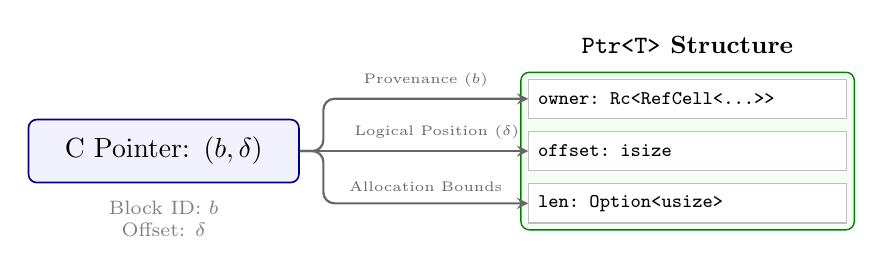
\begin{tikzpicture}[
    node distance=1.0cm and 2.8cm, % 缩小纵向和横向间距，使图形更紧凑
    % 样式定义
    box/.style={rectangle, draw=blue!50!black, fill=blue!5, text width=3.2cm, text centered, rounded corners=3pt, minimum height=0.8cm, line width=0.6pt},
    struct/.style={rectangle, draw=green!50!black, fill=green!5, text width=4cm, minimum height=2cm, rounded corners=3pt, line width=0.5pt}, % 高度从3.5缩至2.4
    field/.style={rectangle, draw=gray!50, fill=white, text width=3.8cm, font=\ttfamily\scriptsize, minimum height=0.5cm}, % 减小字段高度
    arrow/.style={-stealth, thick, color=black!60, line width=0.8pt}
]

    % --- 左侧：C Pointer ---
    \node [box] (c_ptr) {C Pointer: $(b, \delta)$};
    \node [below=0.1cm of c_ptr, align=center, font=\scriptsize\color{gray}] {
        Block ID: $b$ \\ 
        Offset: $\delta$
    };

    % --- 右侧：Ptr Structure ---
    \node [struct, right=of c_ptr] (ptr_struct) {};
    \node [above=0.1cm of ptr_struct, font=\bfseries\small] {\texttt{Ptr<T>} Structure};

    % 将中间的 offset 放在正中心，确保与左侧节点完美水平对齐
    \node [field] (f_offset) at (ptr_struct.center) {offset: isize};
    \node [field, above=0.15cm of f_offset] (f_owner) {owner: Rc<RefCell<...>>};
    \node [field, below=0.15cm of f_offset] (f_len) {len: Option<usize>};

    % --- 映射箭头：带圆角的折线，文字交错分布避免重叠 ---
    % 到 owner 的上折线 (先向右走 1.0cm，再向上拐弯)
    \draw [arrow, rounded corners=4pt] (c_ptr.east) -- ++(0.3, 0) |- (f_owner.west) 
        node[pos=0.75, above=0.02cm, font=\tiny] {Provenance ($b$)};
    
    % 到 offset 的直线 (文字在正中央)
    \draw [arrow] (c_ptr.east) -- (f_offset.west) 
        node[pos=0.6, above=0.02cm, font=\tiny] {Logical Position ($\delta$)};
        
    % 到 len 的下折线 (文字贴在下方折线上)
    \draw [arrow, rounded corners=4pt] (c_ptr.east) -- ++(0.3, 0) |- (f_len.west)
        node[pos=0.75, above=0.02cm, font=\tiny] {Allocation Bounds};

\end{tikzpicture}
%% \vspace{0.5em}
\caption{Mapping from C pointers to the unified \texttt{Ptr<T>} abstraction}
\label{fig:memory_mapping}
\vspace{-0.5cm} % 增加下方间距，防止与正文或 Algorithm 挨得太近
\end{figure}


%% \subsection{Motivation: Comparative Analysis with Naive Translation}
%% \label{sec:motivation}

% 插入文字引导
%% To bridge the semantic gap between C and Rust, we first establish a mapping from Clight's block-offset memory model to our \texttt{Ptr<T>} abstraction, as illustrated in Fig. \ref{fig:memory_mapping}. This design ensures that the abstract pointer provenance ($b$) and logical offset ($\delta$) are explicitly tracked and guarded by Rust's runtime safety mechanisms.

% 随后开始 Scenario 分析...
% In the following, we identify three critical scenarios...


\subsection{A Unified Pointer Abstraction}

%% \noindent
%% \begin{minipage}[t]{\textwidth}
%% \begin{lstlisting}[language=Rust, caption={Definition of Unified Pointers}, frame=tlrb]
%% Inductive expr : Type :=
%%     | Econst_int: int -> type -> expr
%%     | Econst_float: float -> type -> expr
%%     | Econst_single: float32 -> type -> expr
%%     | Econst_long: int64 -> type -> expr
%%     | Evar: ident -> type -> expr
%%     | Etempvar: ident -> type -> expr
%%     | Ederef: expr -> type -> expr
%%     | Eaddrof: expr -> type -> expr
%%     | Eunop: unary_op -> expr -> type -> expr
%%     | Ebinop: bin_op -> expr -> expr -> type -> expr
%%     | Ecast: expr -> type -> expr
%%     | Efield: expr -> ident -> type -> expr
%%     | Esizeof: type -> type -> expr
%%     | Ealignof: type -> type -> expr
%% .
%% \end{lstlisting}
%% \label{lst:clight}
%% \end{minipage}

We present \texttt{Ptr<T>}---the polymorphic Rust structure for representing a pointer to an l-value of type \texttt{T}. Its key feature is that it decouples the \textit{view} of memory from the \textit{ownership} of memory. With this, it enables a direct and safe translation of C pointers to Rust by encoding ownership, offset, and bounds information. Roughly speaking, this structure is composed of three fields:
%
\begin{itemize}
\item \textbf{\texttt{owner}: \texttt{Option<Rc<RefCell<Box<[T]> > > >}}. This field encodes the ownership of memory the pointer points to. It denotes a null pointer if the value is \texttt{None}. For non-null pointers, it enables aliasing and mutability through the combination of reference counting (\texttt{Rc}) and interior mutability (\texttt{RefCell}).

\item \textbf{\texttt{offset}: \texttt{isize}}. It encodes the offset to a pointer, indicating that the pointer value is \texttt{p + offset} where \texttt{p} is the base address of the owned memory.
  
\item \textbf{\texttt{len}: \texttt{Option<usize>}}. This is the (dynamic) upper bound of offsets. It is initially derived from \texttt{malloc} and may change according to Split Tree analysis.

\end{itemize}

%% \begin{algorithm}[!ht]
%% \caption{Definition of the \texttt{Ptr<T>} Abstraction}
%% \label{alg:ptr_def}
%% \footnotesize
%% \begin{algorithmic}[1]
%% \Statex \textbf{Struct} \texttt{Ptr<T>}:
%% \State \textbf{field} \texttt{owner}: \texttt{Option<Rc<RefCell<Box<[T]>>>>}
%% \Statex \hspace*{1.5em} $\triangleright$ \textit{Encodes ownership: Option (NULL), Rc (aliasing), RefCell (mutability)}
%% \State \textbf{field} \texttt{offset}: \texttt{isize}
%% \Statex \hspace*{1.5em} $\triangleright$ \textit{Logical cursor position ($p + i$), decoupled from physical address}
%% \State \textbf{field} \texttt{len}: \texttt{Option<usize>}
%% \Statex \hspace*{1.5em} $\triangleright$ \textit{Dynamic bounds derived from Split Tree analysis}
%% \end{algorithmic}
%% % 底部说明
%% % \vspace{0.5em}
%% % \noindent\textit{\footnotesize This structure enables safe translation of C pointers to Rust by encoding ownership, offset, and bounds information.}
%% \end{algorithm}

%% \subsubsection{Operational Semantics.}
By definition, \texttt{Ptr<T>} encapsulates C pointers under Rust constructs. It also provides the following methods that emulate C pointer semantics safely:

\begin{itemize}
    \item \textbf{Memory Allocation (\texttt{alloc} and \texttt{null}).}
    \texttt{Ptr::alloc(i)} allocates an array containing \texttt{i} elements of type \texttt{T} and returns a \texttt{Ptr<T>} pointer. This is a safe version of \texttt{malloc}. Also, \texttt{Ptr::null()} creates and returns a null pointer.

    \item \textbf{Aliasing via clone (\texttt{clone}).} \texttt{clone()} returns an aliasing \texttt{Ptr<T>} by calling \texttt{Rc::clone} internally. Safety of accessing such aliased pointers is enforced at runtime by reference counting in \texttt{Rc} and interior mutability in \texttt{Refcell}.
    \item \textbf{Pointer Arithmetic (\texttt{offset}).} 
    In C, $p + i$ produces a new pointer without affecting the original. The \texttt{offset} method mimics this by returning a new \texttt{Ptr} instance. Crucially, \texttt{offset(i)} updates the \texttt{offset} field (by adding \texttt{i} to it) without modifying the \texttt{owner}. That is, pointer arithmetic is safe by definition, as no memory access occurs at this stage.
    
    \item \textbf{Memory Access (\texttt{load} and \texttt{store}):} 
    Dereferencing is where safety is enforced. A single read (\texttt{load(i)}) or write (\texttt{store(i, v)}) operation has the following steps:
    \begin{enumerate}
        \item \textbf{Null Check:} It unwraps the \texttt{owner} and panics on \texttt{None}. As a result, accessing to null pointers results in a defined behavior (panic). 
        \item \textbf{Borrow Check:} It calls \texttt{RefCell::borrow()}, enforcing Rust's ``multiple readers or only one writer'' rule dynamically. If a conflict occurs (e.g., a re-entrant modification), the program safely panics instead of causing undefined behavior.
        \item \textbf{Bound Check:} It verifies that $p + i$ is within the valid range $[0, len)$.
        \item \textbf{Access:} Finally, read or write happens on the underlying data.
    \end{enumerate}
\end{itemize}

%% To resolve this, we propose a runtime-assisted translation strategy centered on a unified pointer abstraction, \texttt{Ptr<T>}. This section details the data structure definition, its operational semantics, and provides a comparative analysis to demonstrate the correctness of our design.

As we can see, the \texttt{Ptr<T>} abstraction effectively acts as a dynamic runtime layer that simulates C pointer semantics within safe Rust. By leveraging \texttt{Rc} for liveness and \texttt{RefCell} for aliasing, we shift the verification burden from compile-time (which is often impossible for legacy C) to runtime, guaranteeing memory safety without rejecting valid C patterns. %% We elaborate on this point below.

\subsection{A Hybrid Approach to C-to-Rust Translation}

Our approach to C-to-Rust translation combines static analysis of Split Trees and dynamic ownership enforcement provided by Rust. We discuss its necessity through an example that cannot be handled alone by static analysis in traditional approaches (including Split Trees), and then discuss how we solve this problem by exploiting dynamic ownership provided by \texttt{Ptr<T>}.

\begin{lstlisting}[style=mystyle, language=C, caption={A C function with a dynamic pointer offset}, label={lst:c_example}]
void demonstrate_split_tree(int *arr, int dynamic_offset) {
    // Aliasing analyzable statically 
    int *p1 = arr + 0;
    int *p2 = arr + 5;
    *p1 = 10;
    *p2 = 20;

    // Aliasing not statically analyzable due to dynamic offset
    int *p3 = p1 + dynamic_offset;
    *p3 = *p1 + *p2; 
}
\end{lstlisting}

Consider the C function in Listing~\ref{lst:c_example} which exhibits a common scenario involving pointer arithmetic on both static and dynamic offsets. To translate it into safe Rust, we need to make sure that the write operations through pointers (\texttt{*p1 = 10}, \texttt{*p2 = 20}, \texttt{*p3 = *p1 + *p2}) do not violate Rust's requirement on uniqueness of mutable references.
%
Here, the offsets for \texttt{p1} and \texttt{p2} are constants. To convert such pointers, a static analyzer could detect the constant offsets and divide a continuous memory into disjoint memory slices. That is, tools based on pure static analysis (e.g., Split Trees~\cite{Fromherz2024}) would generate slices by calling a method like \texttt{p.split\_at\_mut(i)}, which is responsible for divide a continuous memory into half at index \texttt{i} (i.e., into \texttt{p[0..i-1]} and \texttt{p[i..]}) and transferring the ownership of divided memory to separate variables. This is shown in Listing~\ref{lst:scylla_failure}. As a result, \texttt{p1} and \texttt{p2} now point to disjoint memory and mutation on disjoint memory is allowed by safe Rust's ownership disciplines.

\begin{lstlisting}[style=mystyle, language=Rust, caption={Failure to generate safe Rust code by the split tree algorithm.}, label={lst:scylla_failure}]
fn demonstrate_split_tree_static(arr: *mut i32, dynamic_offset: i32) {
    let (p1_l, p1_r) = arr.split_at_mut(0);
    let (p2_l, p2_r) = p1_r.split_at_mut(5);
    let (p1, p2) = (p2_l, p2_r);
    p1[0] = 10;
    p2[0] = 20;

    // Split tree algorithm cannot tell if the dynamic offset
    // is < 5 or >= 5. Therefore, it cannot decide whether
    // p1 or p2 should be split and how much the offset is.
    let (p3_l, p3_r) = ??.split_at_mut(??);
    ...
}
\end{lstlisting}

However, this approach cannot be applied to \text{p3} to guarantee the safety of subsequent write operation \texttt{*p3 = *p1 + *p2}. To see that, notice that since we do not know the exact value of \texttt{dynamic\_offset}, we do not know whether \texttt{p3} falls into the range of memory owned by \texttt{p1} or \texttt{p2}. Therefore, we do not know which object or offset \texttt{split\_at\_mut} should be applied to. A purely static approach, such as Scylla, would simply reject this valid C program at this point, failing to produce any output.

Our framework solves this problem by detecting the boundaries of applicability of static reasoning and selectively falls back to runtime ownership enforced by \texttt{Ptr<T>}. For example, if there is no \texttt{p3} in Listing~\ref{lst:c_example}, our algorithm makes use of Split Trees as before. Otherwise, it delegates the aliasing resolution to our \texttt{Ptr<T>} abstraction and generates safe Rust code shown in Listing \ref{lst:rust_example}.

\begin{lstlisting}[style=mystyle, language=Rust, caption={Corresponding safe Rust code generated by our framework}, label={lst:rust_example}]
fn demonstrate_split_tree(mut arr: Ptr<i32>, mut dynamic_offset: i32) {
    let mut p1: Ptr<i32> = Ptr::null();
    let mut p2: Ptr<i32> = Ptr::null();
    let mut p3: Ptr<i32> = Ptr::null();
    
    p1 = arr.clone().offset(0 as isize);
    p2 = arr.clone().offset(5 as isize);
    p1.store(0, 10 as i32);
    p2.store(0, 20 as i32);
    
    // Fallback to dynamic tracking
    p3 = p1.clone().offset(dynamic_offset as isize);
    p3.store(0, (p1.clone().load(0) as i32 + p2.clone().load(0) as i32));
}
\end{lstlisting}

Here, dereferences in C are replaced with safe \texttt{load} and \texttt{store} operations. Aliasing of pointers is implemented by \texttt{clone} operations. If \texttt{dynamic\_offset} results in \texttt{p3} overlapping with \texttt{p1} or \texttt{p2} during execution, the underlying \texttt{RefCell} mechanism will dynamically enforce Rust's borrowing rules to prevent undefined behaviors. This hybrid strategy ensures that even the most unpredictable C idioms can be compiled into safe Rust. Moreover, the translation is straightforward and does not rely on any sophisticated static analysis.

\subsection{Critical Cases of Our Translation}

Below we discuss the critical cases of our translation algorithm. To motivate their design, we compare it with the existing approaches.

\vspace{-0.3cm}
\subsubsection{Scenario 1: Mutable Aliasing.}
C permits multiple pointers to alias the same mutable memory. For example, we have the following C code:
%
\begin{lstlisting}[language=C]
int *p = malloc(2 * sizeof(int));
int *q = p; // 'q' is an alias of 'p'
q[0] = 1;   // Modification via 'q'
return p[0]; // Read via 'p', expects 1
\end{lstlisting}
%

A direct translation produces code rejected by the Rust compiler because of non-unique mutable aliasing. A naive fix to this problem may not preserve the original semantics. For example, the following code forces a deep copy of \texttt{Box} to satisfy the type system, breaking the shared memory semantics.
\begin{lstlisting}[language=Rust]
let mut p: Option<Box<[i32]>> = Some(vec![0; 2].into_boxed_slice());
// ERROR: Box does not support shared ownership. 
// Cloning creates a DISTINCT memory block.
let mut q = p.clone(); 
q.as_mut().unwrap()[0] = 1; // Modifies only q's copy.
return p.as_ref().unwrap()[0]; // Returns 0 (original p is unchanged).
\end{lstlisting}

Our approach fixes this problem by using \texttt{Rc}, i.e., cloning \texttt{Ptr} only increments the reference count. Both \texttt{p} and \texttt{q} point to the same \texttt{RefCell}.
\begin{lstlisting}[language=Rust]
let mut p: Ptr<i32> = Ptr::alloc(2);
let mut q = p.clone();  // Shallow copy. Sharing the same RefCell.
q.store(0, 1);          // Modifies the shared memory.
return p.load(0);       // Correctly returns 1.
\end{lstlisting}

\vspace{-0.3cm}
\subsubsection{Scenario 2: Pointer Arithmetic and Memory Ownership}
A common C idiom is to use \texttt{malloc} to allocate heap memory which should be freed later. Pointers to this heap are used for iteration by pointer arithmetic. For example, 
%
\begin{lstlisting}[language=C]
int *p = malloc(2 * sizeof(int));
p = p + 1; // p now points to the 2nd element
*p = 42;   // Writes to alloc[1]
... // the original memory should be freed (if we have tracked it)
\end{lstlisting}

A naive translation using \texttt{Box} to manage the ownership allocated memory is problematic. We cannot simply ``increment'' the box pointer. Using slices (\texttt{p[1..]}) as in the Split Tree algorithm destroys the original ownership information, making correct deallocation problematic (equivalent to \texttt{free(p+1)} in C, which is Undefined Behavior).

To solve this problem, we have separated the offset (in the \texttt{offset} of \texttt{Ptr<T>}) from the ownership information (in the \texttt{owner} field). As a result, a direct translation is possible as follows where the allocated memory is automatically freed by reference counting when its only pointer \texttt{p} goes out of scope.
%
\begin{lstlisting}[language=Rust]
let mut p: Ptr<i32> = Ptr::alloc(2);
p = p.offset(1); // Returns new Ptr { owner: ..., offset: 1 }
p.store(0, 42);  // Internally accesses owner[1 + 0]
// 'p' goes out of scope, Rc's reference counts drops to 0 and Box is freed
\end{lstlisting}

\vspace{-0.3cm}
\subsubsection{Scenario 3: Lifetime Extension.}
In C, pointers can outlive the scope where they were defined if the memory was allocated on the heap. For example,
%
\begin{lstlisting}[language=C]
int *p = NULL;
if (cond) {
  p = malloc(10 * sizeof(int)); // Allocation happens in an inner scope
}
if (p != NULL) { p[0] = 7; } // Accessed in another scope
\end{lstlisting}

A direct translation would try to lift a temporary allocation to an
outer scope, violating Rust's borrowing checking and resulting in a
compilation error.
%
\begin{lstlisting}[language=Rust]
let mut p: Option<&mut [i32]> = None;
if cond {
    let mut tmp = vec![0; 10].into_boxed_slice();
    // ERROR E0597: `tmp` is dropped here while still borrowed.
    p = Some(&mut tmp);
}
\end{lstlisting}

With our approach, \texttt{Ptr::alloc} creates an \texttt{Rc} structure on the heap. Assigning it to \texttt{p} (defined in the outer scope) extends the lifetime of the heap data naturally via reference counting.
%
\begin{lstlisting}[language=Rust]
let mut p: Ptr<i32> = Ptr::null();
if cond {
    p = Ptr::alloc(10); // Ownership shared by 'p', lifetime extended
}
if !p.is_null() { p.store(0, 7); } // Valid access
\end{lstlisting}

%% \subsection{Illustrative Example: Handling Dynamic Aliasing}

%% To demonstrate the practical limitations of purely static pointer analysis and the necessity of our hybrid approach, consider the C function in Listing \ref{lst:c_example}. It exhibits a common real-world scenario involving both predictable and dynamic memory accesses.

%% \begin{lstlisting}[style=mystyle, language=C, caption={A C function with dynamic pointer offsetting.}, label={lst:c_example}]
%% void demonstrate_split_tree(int *arr, int dynamic_offset) {
%%     // Statically analyzable disjoint regions
%%     int *p1 = arr + 0;
%%     int *p2 = arr + 5;
%%     *p1 = 10;
%%     *p2 = 20;

%%     // Complex aliasing: static isolation fails due to dynamic_offset
%%     int *p3 = p1 + dynamic_offset;
%%     *p3 = *p1 + *p2; 
%% }
%% \end{lstlisting}

%% In this snippet, the offsets for \texttt{p1} and \texttt{p2} are constants, which a static analyzer can trivially divide into disjoint memory slices. However, the calculation of \texttt{p3} relies on \texttt{dynamic\_offset}, a parameter strictly unknown until runtime. Consequently, it is mathematically impossible for a compile-time solver to prove that \texttt{p3} does not alias with the regions held by \texttt{p1} or \texttt{p2}. 

%% When facing such unresolvable symbolic constraints, existing static-first tools (e.g., Scylla) or syntactic transpilers (e.g., C2Rust) fail to provide a safe fallback. As illustrated in Listing \ref{lst:scylla_failure}, they are forced to abandon safe references (\texttt{\&mut T}) entirely, degrading the translation into raw pointer arithmetic wrapped in \texttt{unsafe} blocks. This compromise effectively retains C's memory vulnerabilities, defeating the primary purpose of migrating to Rust.

%% \begin{lstlisting}[style=mystyle, language=Rust, caption={The unsafe fallback generated by purely static translators due to unresolvable dynamic aliasing.}, label={lst:scylla_failure}]
%% extern "C" fn demonstrate_split_tree_static(arr: *mut i32, dynamic_offset: i32) {
%%     unsafe {
%%         // Safe slices (&mut [T]) cannot be used because 
%%         // disjointness is statically unprovable
%%         let p1: *mut i32 = arr.offset(0);
%%         let p2: *mut i32 = arr.offset(5);
%%         *p1 = 10;
%%         *p2 = 20;
        
%%         // Degrades to raw pointer arithmetic, losing all safety guarantees
%%         let p3: *mut i32 = p1.offset(dynamic_offset as isize);
%%         *p3 = *p1 + *p2; 
%%     }
%% }
%% \end{lstlisting}

%% Our framework addresses this bottleneck by recognizing the boundaries of static reasoning and proactively transitioning to a runtime-enforced model. Instead of halting translation or emitting hazardous naked pointers, it delegates the aliasing resolution to our \texttt{Ptr<T>} abstraction. Listing \ref{lst:rust_example} displays the generated safe code.

%% \begin{lstlisting}[style=mystyle, language=Rust, caption={The corresponding Rust code generated by our framework, utilizing dynamic fallback.}, label={lst:rust_example}]
%% extern "C" fn demonstrate_split_tree(mut arr: Ptr<i32>, mut dynamic_offset: i32) {
%%         let mut p1: Ptr<i32> = Ptr::null();
%%         let mut p2: Ptr<i32> = Ptr::null();
%%         let mut p3: Ptr<i32> = Ptr::null();
        
%%         p1 = arr.clone().offset(0 as isize);
%%         p2 = arr.clone().offset(5 as isize);
%%         p1.store(0, 10 as i32);
%%         p2.store(0, 20 as i32);
        
%%         // Fallback to dynamic tracking
%%         p3 = p1.clone().offset(dynamic_offset as isize);
%%         p3.store(0, (p1.clone().load(0) as i32 + p2.clone().load(0) as i32) as i32);
%% }
%% \end{lstlisting}

%% Here, unchecked dereferences are strictly replaced with mediated \texttt{.load()} and \texttt{.store()} calls, and the complex aliasing relationships are legally maintained via explicit \texttt{.clone()} operations. If \texttt{dynamic\_offset} ultimately causes \texttt{p3} to overlap with \texttt{p1} or \texttt{p2} during execution, the underlying \texttt{RefCell} mechanism will dynamically enforce Rust's borrowing rules to prevent data races. This hybrid strategy ensures that even the most unpredictable C idioms can be compiled into 100\% Safe Rust without undefined behaviors.
%\subsection{Advanced Translation Features}

\subsubsection{Decay and Casting of Arrays.}
%
To integrate arrays into our framework, we need to encapsulate their accesses beneath public traits using a minimum amount of unsafe code. As a result, unsafe code will only occur in what we called the ``runtime library'' (see Sec.~\ref{ssec:runtime}) and will never occur at user level.
%
For example, in C, arrays implicitly decay to pointers. To emulate this in Rust, where arrays \texttt{[T; N]} and pointers are distinct, we introduce the \texttt{ArrayPtrCastExt} trait.
\begin{lstlisting}[language=Rust]
pub trait ArrayPtrCastExt { fn cast<U>(&self) -> Ptr<U>; }
impl<T, const N: usize> ArrayPtrCastExt for [T; N] {
    fn cast<U>(&self) -> Ptr<U> {
        // Creates a Ptr view from a raw pointer to the stack array.
         unsafe { Ptr::from_raw_parts(self.as_ptr() as *mut U, N) }
    }
}
\end{lstlisting}
This allows generated code to seamlessly treat stack arrays as \texttt{Ptr} objects, enabling calls like \texttt{arr.cast::<i32>().offset(2)}.

\subsubsection{Safe Initialization.}
Safe Rust requires all variables to be initialized before use. Clight allows uninitialized declarations. We bridge this gap using a recursive initialization strategy \texttt{array\_default}, which internally constructs a zero-initialized array and exposes it safely, satisfying Rust's initialization analysis.

%% \subsection{Summary of Improvements}




\section{Overview of the System}
\label{sec:overview}

Our system \textbf{Clight2Rust} (as shown in Figure~\ref{fig:workflow}) intercepts the compilation pipeline of the CompCert compiler \cite{Leroy2009} at the \emph{Clight} intermediate representation and redirects the target to \emph{Rustlight} \cite{Wu2025}. The core of the system is the translation pass defined in the Coq file \texttt{Clight2Rustlight.v}, which implements a formal transformation that realizes the key ideas in Sec.~\ref{sec:algorithm}. After that, Rustlight programs are printed into Rust source code and compiled together with our runtime library to generate executable code. A more in-depth discussion of the implementation of \textbf{Clight2Rust} is given in Appendix~\ref{sec:impl}.

\begin{figure}[htbp]
\vspace{-0.4cm}  
\centering
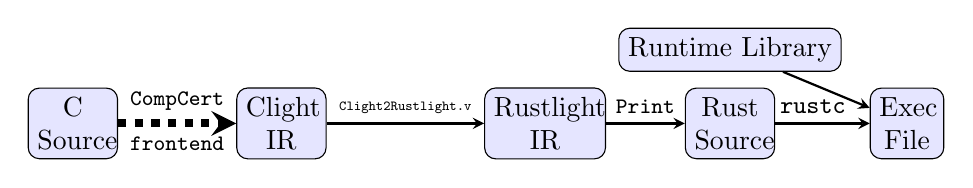
\begin{tikzpicture}[node distance=0.8cm, auto,
    block/.style={rectangle, draw, fill=blue!10, text centered, rounded corners, minimum height=0.5cm},
    arrow/.style={thick,->,>=stealth}]
    
    % --- 主流程节点 ---
    \node [block, text width = 0.9cm] (csrc) {C Source};
    \node [block, text width = 0.9cm, right=1.5 of csrc] (clight) {Clight IR};
    \node [block, text width = 1.3cm, right=2 of clight] (rustlight) {Rustlight IR};
    \node [block, text width = 0.9cm, right=1of rustlight] (rssrc) {Rust Source};
    \node [block, text width = 0.7cm, right=1.2 of rssrc] (binary) {Exec File};
    
    % --- 新增节点：定位在 Rust Source 上方 ---
    % 使用 above=of rssrc 将其放在 Rust Source 正上方
    \node [block, above=of rssrc, above=0.2cm of rssrc] (runtime) {Runtime Library};
    
    % --- 描述文字 ---
    %% \node [text width=2.5cm, align=center, below=0.2cm of clight] {\footnotesize (CompCert Frontend)};
    %% \node [text width=2.5cm, align=center, below=0.4cm of rustlight] {\footnotesize (\textbf{Clight2Rustlight.v})};
    %% \node [text width=2.5cm, align=center, below=0.1cm of rssrc] {\footnotesize (PrintRustlight.ml)};
    
    % --- 箭头连接 ---
    % 1. 主流程
    \draw [arrow, line width = 0.1cm, dashed] (csrc) --
    node[above, font=\footnotesize] {\texttt{CompCert}}
    node[below, font=\footnotesize] {\texttt{frontend}}
    (clight);
    
    \draw [arrow] (clight) --
    node[above, font=\tiny] {\texttt{Clight2Rustlight.v}}
    (rustlight);
    
    \draw [arrow] (rustlight) --
    node[above, font=\footnotesize] {\texttt{Print}}
    (rssrc);
    
    % 2. Rust Source -> Executable (标注 rustc)
    % 为了让标签不重叠，我们可以把标签放在这条线上
    \draw [arrow] (rssrc) -- node[above, pos=0.4, font=\small] {\texttt{rustc}} (binary);
    
    % 3. Runtime Library -> Executable
    % 从上方节点直接指向 binary
    \draw [arrow] (runtime) -- (binary);
    
\end{tikzpicture}

\caption{End-to-End Translation Pipeline of Clight2Rust}
\label{fig:workflow}
\vspace{-0.7cm}
\end{figure}

\subsection{Translation Architecture}

The translation in \texttt{Clight2Rustlight.v} is structured as a \emph{bottom-up recursive} function, processing the Clight Abstract Syntax Tree (AST) from the leaves (expressions) to the root (the entire program). This process is implemented with a monadic context (using the \texttt{res} error monad in Rocq) to handle potential translation failures and propagate the compilation environment (e.g., type definitions and global symbols).
%
The transformation proceeds in four phases, as follows.

\textbf{Phase 1: Expression and Pointer Transformation (\texttt{transl\_expr}).}
%
This is the most critical phase, which materializes the ideas for turning Clight expressions into the \texttt{Ptr<T>} API calls formulated in Section 3. Clight distinguishes between \textit{l-values} (locations) and \textit{r-values} (values), allowing implicit conversions (decay). In contrast, Rustlight requires explicit method calls for memory accesses.
%
The function \texttt{transl\_expr} recursively traverses Clight expressions as shown in Algorithm~\ref{alg:translation}. The complex pointer operations are handled as follows:
\begin{itemize}
    \item \textbf{Recursive Composition:} For a nested expression like \texttt{**p} (double dereference), the translator first recursively calls \texttt{transl\_expr(p)} to resolve the inner pointer, producing a Rustlight expression representing a \texttt{Ptr<T>}. It then generates a \texttt{load} operation on this result to get the inner address, and finally generates another \texttt{load} for the outer dereference.
    \item \textbf{Explicit Memory Access:} The translation explicitly distinguishes between pointer arithmetic and memory access.
    \begin{itemize}
        \item \texttt{Ebinop(Oadd, p, i)} is translated to \texttt{p.offset(i)}. This merely calculates a new view (updating the offset field) without touching memory.
        \item \texttt{Ederef(p)} is translated into \texttt{p.load(0)}. This forces a runtime borrow check and performs memory read.
        \item \texttt{Efield(p, id)} (struct access) is translated into \texttt{(p.load(0)).id}, effectively loading the struct instance before accessing its field.
    \end{itemize}
\end{itemize}


\begin{algorithm}[!ht]
\caption{Core Recursive Translation Logic in \texttt{transl\_expr}}
\label{alg:translation}
\footnotesize
\begin{algorithmic}[1]
\Require A Clight expression $e$
\Ensure A translated Rustlight expression or an error

\Statex \textbf{Function} \texttt{transl\_expr}($e$):
\State \textbf{match} $e$ \textbf{with}
    \State \quad $|$ \texttt{Econst\_int}($n, \_$): \quad\quad \textbf{return} $\texttt{OK}(\texttt{Rconst\_i32 } n)$;
    \State \quad $|$ \texttt{Etempvar}($id, \_$): \quad\quad \textbf{return} $\texttt{OK}(\texttt{Rvar } id)$;
    
    \State \quad $|$ \texttt{Ebinop(Oadd, } $e_1, e_2, \_$\texttt{)}: \Comment{Pointer Arithmetic}
        \State \quad\quad $r_1 \gets \texttt{transl\_expr}(e_1)$; 
        \quad $r_2 \gets \texttt{transl\_expr}(e_2)$;
        \State \quad\quad \textbf{return} $\texttt{OK}(\texttt{Rcall } (\texttt{Rmethod } r_1 \texttt{ "offset"}) \ [r_2])$;
    
    \State \quad $|$ \texttt{Ederef(}$e_1, \_$\texttt{)}: \Comment{Dereference}
        \State \quad\quad $r_1 \gets \texttt{transl\_expr}(e_1)$;
        \quad \textbf{return} $\texttt{OK}(\texttt{Rcall } (\texttt{Rmethod } r_1 \texttt{ "load"}) \ [0])$;
    
    \State \quad $|$ \texttt{Efield(}$e_1, id, \_$\texttt{)}: \Comment{Field Access}
        \State \quad\quad $r_1 \gets \texttt{transl\_expr}(e_1)$;
        \quad $struct\_val \gets \texttt{Rcall } (\texttt{Rmethod } r_1 \texttt{ "load"}) \ [0]$;
        \State \quad\quad \textbf{return} $\texttt{OK}(\texttt{Rfield } struct\_val, id)$;

    \State \quad $|$ \_: 
     ...
\State \textbf{end match}
\end{algorithmic}

% 将描述文字放在算法底部，使用 \caption* 生成无编号的副标题样式
% 如果不想用 caption 包，也可以直接用 \vspace{2mm} \noindent \textit{...}
% \caption*{This algorithm depicts the recursive lowering logic described above.}
\end{algorithm}

\textbf{Phase 2: Statement Mapping (\texttt{transl\_statement}).}
This phase handles control flow and side effects after translating expressions.
\begin{itemize}
    \item \textbf{Assignments:} An assignment \texttt{*p = v} in C involves evaluating the left-hand side to a location and the right-hand side to a value. Our translator converts this into a method call: \texttt{p.store(0, v)}. This ensures all memory writes go through the dynamic safety checks provided by the \texttt{Ptr<T>} abstraction.
    \item \textbf{Control Flow normalization:} C loops (e.g., \texttt{Sloop}, \texttt{Swhile} in Clight) are normalized into Rust's infinite \texttt{loop} structure combined with \texttt{match} statements to handle \texttt{break} and \texttt{continue} conditions, bridging the semantic gap between C's structured jumps and Rust's expression-based control flow.
\end{itemize}

\textbf{Phase 3: Function Processing (\texttt{transl\_function}).}
The function-level translation creates a local environment and iterates over the function's parameters and local variable declarations.
\begin{itemize}
    \item \textbf{Stack Allocation:} Local arrays and structs in C are identified. The translator generates corresponding Rust initialization code (using \texttt{array\_default}) to ensure that all stack variables are initialized before use, satisfying Rust's definite initialization requirement.
    \item \textbf{Signature Matching:} The function signature is transformed, mapping C types to Rustlight types (e.g., \texttt{int} $\to$ \texttt{i32}, \texttt{char*} $\to$ \texttt{Ptr<i8>}).
\end{itemize}

\textbf{Phase 4: Whole-Program Assembly (\texttt{trans\_program}).}
Finally, the function \texttt{trans\_program} aggregates all translated functions and global variables.
A specific detail in our implementation (as in \texttt{Clight2Rustlight.v}) is the explicit injection of external definitions for \texttt{malloc} and \texttt{free}. Since these are built-in primitives in C, our pass checks for their existence and injects the corresponding \texttt{External} function definitions into the Rustlight AST. This ensures that the generated code links correctly against our runtime library.

\subsection{Printing and Runtime}
\label{ssec:runtime}
To produce Rust source code from Rustlight. We design an OCaml printer (\texttt{PrintRustlight.ml}) to traverse the Rustlight AST and print Rust code, which handles syntactic sugar, module imports, indentation, etc.
Moreover, we design a Runtime Library to provide the concrete implementation of \texttt{Ptr<T>}, \texttt{malloc}, and \texttt{free}, serving as the trusted execution environment for our translation.


\section{Evaluation}
\label{sec:eval}

In this section, we evaluate \textbf{Clight2Rust} to answer the following questions:
\begin{itemize}
    \item \textbf{RQ1 (Compatibility \& Correctness):} Can our tool translate diverse C programs into valid safe Rust code, and do they produce correct outputs?
    \item \textbf{RQ2 (Performance):} What is the runtime overhead introduced by our \texttt{Ptr<T>} abstraction and safety checks compared to native C?
\end{itemize}

\subsection{Experimental Setup}

\subsubsection{Environment.}
All experiments were conducted on an Apple MacBook Air equipped with an \textbf{Apple M4} chip and \textbf{16 GB} of RAM, running \textbf{macOS 15.2 (Build 25C56)}. The software toolchain includes:
\begin{itemize}
    \item \textbf{C Compiler:} Apple clang version 17.0.0 (targeting \texttt{arm64-apple-darwin}).
    \item \textbf{Rust Compiler:} \texttt{rustc} version 1.93.0-nightly (2025-10-25).
    \item \textbf{Coq:} Version 8.12.0.
    \item \textbf{Optimization:} Both C and Rust are compiled with level 2 optimizations (\texttt{-O2} for GCC/Clang, \texttt{-O} for Rustc) to ensure a fair performance comparison.
\end{itemize}

\subsubsection{Benchmarks.}
We evaluated our tool on the standard CompCert test suite (\texttt{test/c}), which contains 24 benchmarks ranging from computational kernels (e.g., \texttt{fft}, \texttt{aes}) to data structure manipulations (e.g., \texttt{binarytrees}, \texttt{lists}). 
%% Two benchmarks, \texttt{knucleotide} and \texttt{mandelbrot}, failed to run in the C baseline environment (likely due to missing input files) and were excluded from the comparative analysis, leaving a total of 22 valid benchmarks.

\subsection{Correctness and Compatibility (RQ1)}

We consider a translation successful if the generated Rust code compiles without errors and produces output identical to the C reference implementation compiled using GCC on representative inputs.
As shown in Table \ref{tab:results_final}, our tool successfully translated and executed \emph{all} benchmarks, achieving a success rate of \emph{100\%}. Since CompCert's test suite is designed to cover all the C features that CompCert's C subset could support. This demonstrates that our \texttt{Ptr<T>} abstraction is capable of handling at least CompCert's subset of C, which includes a wide variety of C constructs, such as pointer arithmetic, recursive structures, and callbacks.

\begin{center}
\captionof{table}{Translation Results and Performance Comparison.}
\label{tab:results_final}
\centering
\resizebox{\textwidth}{!}{%
\begin{tabular}{|l|c|c|c|c|r|}
\hline
\textbf{Benchmark} & \textbf{Category} & \textbf{Success} & \textbf{C Time (s)} & \textbf{Rust Time (s)} & \textbf{Overhead} \\
\hline
\texttt{binarytrees} & Allocation    & \textbf{OK} & 0.8918 & 0.6009 & \textbf{0.67x} \\
\texttt{bisect}      & Control Flow  & \textbf{OK} & 0.5666 & 0.5223 & \textbf{0.92x} \\
\texttt{mandelbrot}  & Fractal       & \textbf{OK} & 0.4439 & 0.4334 & \textbf{0.98x} \\
\texttt{fib}         & Recursion     & \textbf{OK} & 0.3919 & 0.3917 & 1.00x \\
\texttt{integr}      & Math          & \textbf{OK} & 0.3846 & 0.4016 & 1.04x \\
\texttt{perlin}      & FP Arith      & \textbf{OK} & 0.4036 & 0.4744 & 1.18x \\
\texttt{sha1}        & Crypto        & \textbf{OK} & 0.4447 & 0.5582 & 1.26x \\
\texttt{qsort}       & Callbacks     & \textbf{OK} & 0.5000 & 0.6405 & 1.28x \\
\texttt{nsieve}      & Array Sieve   & \textbf{OK} & 0.4693 & 0.6517 & 1.39x \\
\texttt{aes}         & Crypto        & \textbf{OK} & 0.6035 & 0.8726 & 1.45x \\
\texttt{fft}         & DSP           & \textbf{OK} & 0.4805 & 0.6954 & 1.45x \\
\texttt{almabench}   & Logic         & \textbf{OK} & 0.4101 & 0.6054 & 1.48x \\
\texttt{nsievebits}  & Bits          & \textbf{OK} & 0.5516 & 0.8283 & 1.50x \\
\texttt{vmach}       & Virtual Mach. & \textbf{OK} & 0.4532 & 0.7730 & 1.71x \\
\texttt{fftsp}       & DSP (Float)   & \textbf{OK} & 0.4021 & 0.7527 & 1.87x \\
\texttt{fftw}        & DSP           & \textbf{OK} & 0.4312 & 0.8103 & 1.88x \\
\texttt{siphash24}   & Hashing       & \textbf{OK} & 0.4556 & 0.8583 & 1.88x \\
\texttt{spectral}    & Math          & \textbf{OK} & 0.4403 & 0.8828 & 2.00x \\
\texttt{knucleotide} & String        & \textbf{OK} & 0.4560 & 1.0316 & 2.26x \\
\texttt{sha3}        & Bitwise       & \textbf{OK} & 0.3838 & 0.9529 & 2.48x \\
\texttt{chomp}       & Game          & \textbf{OK} & 0.4822 & 1.2488 & 2.59x \\
\texttt{nbody}       & Physics       & \textbf{OK} & 0.4560 & 1.1994 & 2.63x \\
\texttt{lists}       & Pointers      & \textbf{OK} & 0.4265 & 1.1248 & 2.64x \\
\texttt{fannkuch}    & Permutation   & \textbf{OK} & 0.5414 & 1.8178 & 3.36x \\
\hline
\end{tabular}%
}
\end{center}
%% \subsubsection{Success Rate.}

\subsection{Performance (RQ2)}

Table \ref{tab:results_final} details the execution time. In this table, the mean overhead for the benchmarks is \emph{1.70x}. We analyze the performance overhead as follows:
%
\begin{itemize}
    \item \textbf{Comparable Performance ($<1.0$x):} surprisingly, benchmarks like \texttt{binarytrees}, \texttt{bisect} and \texttt{mandelbrot} ran faster in Rust (approximately 0.9x). This suggests that for logic dominated by simple arithmetic or recursion, the Rust compiler (LLVM) may perform more aggressive optimizations (e.g., tail-call optimization or inlining) than the reference Clang build, or that our slice-based access allows for better vectorization in specific loops.
    
    \item \textbf{Moderate Overhead ($1.2$x - $2.0$x):} Most computation-intensive benchmarks (e.g., \texttt{aes}, \texttt{fft}) fall in this range. The overhead comes from the extra instructions required for \texttt{Ptr} offset calculations and the dynamic bounds checks embedded in slice accesses.
    
    \item \textbf{High Overhead ($>2.5$x):} The observed performance degradation (approximately 3x) in benchmarks like \texttt{lists}, \texttt{chomp}, and \texttt{fannkuch} stems from the overhead of safety-encapsulated pointer operations. In C, memory access is a direct pointer dereference. In our translated Rust code, each access through the \texttt{Ptr<T>} abstraction results in heavy runtime cost. We conjecture the costs come from (1) Dynamic Borrowing: the use of \texttt{Rc<RefCell<Box<[T]> > >} requires pattern matching, index calculation, and \texttt{RefCell}'s dynamic borrow counting for every load and store operation, incurring a significant cost in hot loops; (2) Inefficient Field Updates: the current translation for structure fields employs a ``load-modify-store'' pattern, which triggers unnecessary cloning of the entire structure rather than in-place modification.
\end{itemize}

\subsection{Scope and Interpretation}
It is crucial to interpret the 100\% success rate within the defined scope. Our benchmarks are drawn from the CompCert test suite, which is designed to exercise the features of its formally verified C subset (Clight). Therefore, the evaluation validates that our translation is complete and correct for this specific, well-behaved subset. It does not constitute a claim of full coverage for arbitrary, GNU-extended C code. As detailed in Section~5, our approach maintains a clear boundary: programs must be expressible in Clight, supported by our translation rules, and compatible with our runtime library's pointer model.

\subsection{Summary}
The evaluation shows that \textbf{Clight2Rust} produces safe Rust code that is functionally correct for standard benchmarks. While the strict enforcement of memory safety introduces an average overhead of 1.70x, this is a reasonable trade-off for the guarantee of memory safety, especially considering that no \texttt{unsafe} blocks are used in the generated code (excluding the runtime library).

\section{Discussions and Limitations}
\label{sec:discuss}

While our approach successfully bridges a significant semantic gap for a well-defined subset of C, it involves deliberate trade-offs in terms of generality, performance, and the depth of static guarantees.

Our translation pipeline inherits its front-end from CompCert, which accepts a large but carefully defined subset of C (Clight) and excludes most compiler-specific extensions (e.g., GNU C nested functions, inline assembly). Consequently, any input C program must first be valid within the CompCert/Clight ecosystem. Further restrictions are imposed by our own translation layer (\texttt{Clight2Rustlight.v}). While we handle the core imperative constructs, several statement and expression forms are not yet directly supported and are either rewritten (e.g., \texttt{switch} is lowered to \texttt{if-else} chains) or explicitly rejected. Examples of currently unsupported patterns include \texttt{goto} statements, taking the address of a unary operation or a \texttt{sizeof} expression, and certain complex l-value casts. These limitations mean the tool is most robust when translating structured, idiomatic C.  Our current evaluation uses the CompCert test suite precisely because it falls well within this supported syntactic space.  For multi-file C projects, our compiler currently processes each source file individually; the resulting Rust files are then assembled into a single crate by an external script that rewrites cross-file \texttt{extern "C"} declarations.  While this suffices for the PolyBench suite, it is an engineering workaround rather than a native handling of C's translation-unit linkage, and subtle issues with internal linkage or macro expansions can still arise.

In terms of trust, our end-to-end correctness relies on several components.  First, we rely on the correctness of the C standard library. We assume that the external C standard library functions (e.g., \texttt{malloc} and \texttt{printf}) behave according to their specifications. Any undefined behavior within a library may break the safety of our code. Second, the correctness of \texttt{unsafe} blocks within our runtime library (\texttt{runtime/ptr.rs}) is crucial for ensuring safety. For example, we assume that the \texttt{cast} operations between different types (via \texttt{ArrayPtrCastExt}) respect memory layout.  Moreover, the pretty-printer (\texttt{PrintRustlight.ml}) contains a significant amount of non-trivial logic for initialization, control-flow reconstruction, and type casting; bugs in these passes can silently lead to generated code that compiles but behaves differently from the original C.  A formally verified implementation of the standard and runtime libraries (using tools like RustBelt~\cite{Jung2017}) would further reduce this trusted computing base.

A key design decision in Clight2Rust is the use of the \texttt{Ptr<T>} abstraction, which utilizes reference counting (\texttt{Rc}) and interior mutability (\texttt{RefCell}) to effectively defer borrow checking to runtime. This enables a direct translation of many forms of C pointer operations into safe Rust code without solely relying on complex static analysis. For example, ``spaghetti pointers'' that are common in legacy C code, which are impossible to express with standard \texttt{\&mut T} references, could be translated with our approach. However, the resulting code, while safe, is not ``idiomatic'' Rust which in many cases enforces borrow rules statically. Another drawback is that the runtime borrow checking introduces execution overhead as we discussed in evaluation.  A particularly fragile point is the treatment of arrays.  C implicitly decays arrays to pointers, but in our model the translator must decide whether to \texttt{load} an entire array (creating a copy on the stack) or to obtain a view via \texttt{offset}/\texttt{row}.  When large multi-dimensional arrays are involved, an incorrect choice can lead to stack overflows or silently incorrect results, even though the generated Rust compiles successfully.  Our current heuristics handle the CompCert test suite well, but this aspect remains one of the most brittle parts of the translation.  Similarly, our support for dynamic memory management (\texttt{malloc}, \texttt{free}, \texttt{realloc}, etc.) and C standard library functions is achieved through a combination of runtime wrappers and pattern-based recognition in the printer.  Coverage is not yet complete: for instance, \texttt{free} calls that do not follow the expected pattern are simply commented out in the output, and less common library functions or variadic functions with complex argument promotions are not yet robustly supported.

As readers may observe, we have adopted a very conservative approach to handling undefined behaviors. That is, any memory error (e.g., out-of-bounds access) would trigger a panic at runtime. Although this prevents undefined behaviors, it is also not desirable in many situations where crashes during execution could be fatal. A particular such case is the violation of uniqueness of mutable references, which ideally should be caught by borrow checker statically, but instead is delayed to run time in our approach.  Furthermore, the runtime checks on bounds rely on length information that is carried inside \texttt{Ptr<T>}; certain pointer arithmetic operations (e.g., offsetting beyond the statically known extent) can lose accurate length information, after which dynamic bounds checking degrades to a best-effort basis.

Finally, our current implementation has limited support for concurrency and stack data. We use \texttt{Rc} and \texttt{RefCell}, which are not thread safe. Translating concurrent C code would require replacing these with thread-safe primitives like \texttt{Arc} and \texttt{RwLock}. We also rely on \texttt{Rc<RefCell<...> >} which forces all pointed-to data to reside on the heap, prohibiting pointers to stack-allocated variables without performing a deep copy.

All the above problems could be solved by migrating to an approach that employs more aggressive static analysis when possible. With such analysis, it will be possible to turn \texttt{Rc<RefCell<...> >} into standard \texttt{Box} or stack-allocated data. With this change, runtime panics caused by dynamic borrow checking and other undefined behaviors may be prevented at compile time. We plan to carry out this enhancement in the future.

\section{Conclusion}
\label{sec:concl}

We have presented \textbf{Clight2Rust}, a lightweight framework for translating a subset of C programs into safe Rust by leveraging the precise semantics of CompCert's Clight language and utilizing reference counting and interior mutability in Rust.
As a result, we are able to translate a wide range of C programs into safe Rust without relying on complex static analysis, which was not possible before. We have implemented a translation pipeline integrated into CompCert that handles practical challenges like initialization, variadic functions, and FFI callbacks. An evaluation on standard benchmarks shows that our tool achieves high compatibility and correctness, producing executables that match the behavior of GCC-compiled code while enforcing memory safety.

In the future, we plan to design an even more hybrid approach by integrating aggressive static analysis, in order to turn dynamic borrow checking into static checking, thereby eliminating runtime panics and reducing runtime overhead. To support more real-world applications, we also plan to expand the coverage of our tool by extending the standard library support, i.e., providing safe Rust implementation for a wider range of \texttt{libc} functions (e.g., file I/O, string manipulation). To address the heavy dependency on heap memory, we plan to explore a new pointer abstraction based on interior mutability using \texttt{\&[Cell<T>]}. Recent work on GhostCell \cite{Yanovski2021} shows that separating data permissions from data representation allows for safe and aliased mutation. By mapping C pointers to shared references of \texttt{Cell} slices, we can potentially support pointers to stack variables and eliminate the overhead of \texttt{RefCell}, thereby moving closer to true zero-cost abstractions while maintaining safety guarantees.
%
Finally, we would like to establish a fully formalized semantic preservation proof from Clight to Rustlight, thereby creating a verified C-to-Rust translator.


% ------------------------
% Reference section
% ------------------------
\bibliography{reference} % Assumes your .bib file is named reference.bib

% ------------------------
% Appendix section
% ------------------------
% ------------------------------------------------------------------
% 参考文献之后添加附录
% ------------------------------------------------------------------
\newpage % 建议另起一页
\appendix

\section{Implementation}
\label{sec:impl}

Our implementation is integrated into the CompCert framework. It consists of a formal specification in Rocq, defining the translation logic from Clight to Rustlight, and an OCaml/Rust backend that synthesizes executable source code. 

% \subsection{Semantics and Specification}

% The formal verification relies on two key components: the target language definition and the translation relation.

% \subsubsection{Target Semantics (Rustlight).}
% We target \textbf{Rustlight}, a formalized intermediate representation of Safe Rust developed by Wu et al. Rustlight models the core ownership and borrowing mechanisms of Rust, providing a semantic foundation for our translation. It defines the abstract syntax for Rust items (structs, functions, enums) and statements. Our contribution lies in adapting the \texttt{Clight} memory model to match Rustlight's type system, specifically mapping CompCert's block-offset pointers to Rustlight's abstract references.

\subsection{Translation Logic}
This Coq module(\texttt{Clight2Rustlight.v}) implements the core logic of our approach. It defines a function \texttt{trans\_program} that traverses the Clight AST.
\begin{itemize}
    \item \textbf{Type Translation:} We define a mapping $\tau_c \to \tau_r$, where C arrays are mapped to Rust arrays or slices depending on the context (as analyzed by the Split Tree algorithm), and C structs are mapped to Rust structs with \texttt{Cell}-wrapped fields where interior mutability is required.
    \item \textbf{Statement Translation:} The translation recursively converts C statements. Critical operations such as pointer dereferencing (\texttt{*p}) and arithmetic (\texttt{p+i}) are lowered into method calls on our \texttt{Ptr<T>} abstraction (e.g., \texttt{ptr\_load}, \texttt{ptr\_offset}).
    \item \textbf{Undefined Behavior:} The translation assumes the source C program is free of undefined behavior (UB). For constructs that are valid in C but indistinguishable from errors in Safe Rust (e.g., out-of-bound access), our generated code relies on Rust's runtime panic mechanism to halt execution safely.
\end{itemize}

% \subsection{Proof Strategy}

% The ultimate goal of our formalization is to prove a \textbf{semantic preservation theorem}, asserting that if a source Clight program behaves safely, the generated Rustlight program exhibits equivalent behavior.

% \subsubsection{Simulation Relation.}
% We formulate the correctness proof as a forward simulation between the execution traces of Clight and Rustlight.
% $$
% \forall S, S', T. \quad (S \xrightarrow{C} S') \land \text{match}(S, T) \implies \exists T'. (T \xrightarrow{R} T') \land \text{match}(S', T')
% $$
% Here, $\text{match}(S, T)$ represents the invariant that memory states in Clight (blocks and offsets) are consistently represented by the \texttt{Ptr} values and memory snapshots in Rustlight.

% \subsubsection{Current Status.}
% In the current version of \textbf{Clight2Rustlight}, the definitions of syntax, semantics, and the translation functions are fully mechanized in Coq. The simulation proofs and the specific lemmas regarding memory injection are currently admitted (\texttt{Admitted} in Coq). The rigorous definition of these properties serves as a specification for our implementation, ensuring that the algorithmic design (Chapter \ref{sec:algorithm}) is theoretically sound, even though the complete machine-checked proof is left for future work.

\subsection{Printing and Runtime Support}
\label{ssec:print-runtime}

A significant portion of our contribution is the bridge between the formalized AST and the actual compiling Rust code. This is handled by the OCaml printers and the Rust runtime library.

\subsubsection{The OCaml Printers.}
We implement the code generation in OCaml files \texttt{PrintRustlight.ml} and \texttt{PrintRustsyntax.ml}.
\begin{itemize}
    \item \textbf{Syntactic Sugar \& Control Flow:} Since Rustlight is a simplified IR, the printer reconstructs idiomatic Rust syntax. It handles the conversion of C-style `for' loops into Rust `loop' or `while' constructs and manages the lexical scoping of variables to satisfy Rust's liveness requirements.
    \item \textbf{Initialization Consumption:} Safe Rust requires all variables to be initialized. \texttt{PrintRustsyntax.ml} implements a ``consumption algorithm'' for struct and array initialization. It topologically sorts field initializers to match Rust's struct literal syntax (\texttt{Struct \{ field: val, ... \}}) and generates \texttt{Default::default()} for unspecified fields to mimic C's zero-initialization behavior.
    \item \textbf{Standard Library Wrappers:} The printer automatically injects safe wrappers for common C library functions like \texttt{qsort}, \texttt{bsearch}, \texttt{printf}, and \texttt{scanf}. For instance, \texttt{qsort} is translated into a generic function that takes a closure, bridging the gap between C function pointers and Rust traits.
\end{itemize}

\subsubsection{The Runtime Library.}
The generated code links against a handwritten runtime library (\texttt{runtime/}), which provides the concrete implementation of the primitives assumed in the formalization.

\begin{itemize}
    \item \textbf{Pointer Implementation (\texttt{ptr.rs}):} This file implements the \texttt{Ptr<T>} struct discussed in Section \ref{sec:algorithm}. It uses \texttt{unsafe} internally to perform raw pointer arithmetic and casts (e.g., casting \texttt{*mut u8} to \texttt{*mut T}) but exposes a strictly safe API to the generated code. It serves as the trusted boundary where memory safety invariants are dynamically checked (e.g., via \texttt{RefCell} borrowing rules and bounds checking).
    \item \textbf{FFI and Callbacks (\texttt{callback.rs}):} To support C-style callbacks (e.g., in \texttt{qsort}), we implement a \texttt{CallbackSlot} mechanism. Since Rust closures cannot be directly cast to C function pointers, we use a global thread-local storage to temporarily hold the closure and pass a static ``trampoline'' function to the C side. This ensures that the context-sensitive Rust closure is safely invoked when the C library calls the function pointer.
\end{itemize}

This split architecture—verified translation logic combined with a robust runtime system—allows us to produce code that is both formally grounded and practically executable.

\end{document}
